\documentclass[12pt]{article}

\usepackage[a4paper, margin=2.5cm]{geometry}
\usepackage{graphicx}
\usepackage{fontenc}
\usepackage{inputenc}
\usepackage{setspace}
\usepackage{hyperref}
\usepackage{setspace}
\usepackage{booktabs}
\usepackage{caption}
\usepackage{subcaption}
\usepackage{amsmath}
\usepackage{hyperref}
\usepackage{circuitikz}
\begin{document}

\begin{titlepage}
    \centering

    % University logo
    
\includegraphics[width=0.45\textwidth]{images/ozu_logo.png}\\[3cm]

    % Course
    {\large \textbf{EE 350 -- Electronics II}}\\[1cm]

    % Semester
    {\large \textbf{Spring 2025/26}}\\[1cm]

    % Lab number
    {\large \textbf{TERM PROJECT}}\\[1cm]

    % Lab title
    {\large \textbf{Design of a Differential Cross-Coupled Oscillator}}\\[5cm]

    % Submission info
    \begin{center}
        {\normalsize \textbf{Submitted by:} Ömer Faruk AVCI}\\[0.4cm]
        {\normalsize \textbf{Student ID:} S034113}\\[0.4cm]
        {\normalsize \textbf{Date of Submission:} 05.04.2026}
    \end{center}

\end{titlepage}

%------------------------------
% Introduction starts here
%------------------------------
\section*{1 Introduction}
The design of stable high-frequency signal sources is a fundamental requirement in modern wireless communication systems. This term project details the design and implementation of a 350 MHz differential cross-coupled LC oscillator using a 0.35 $\mu$m CMOS process. To ensure the performance is independent of environmental factors, the system incorporates a Bandgap Reference (BGR) generator that provides a temperature-stable 0.5 mA bias current.\\
\newline
\noindent
The primary design objectives include achieving a single-ended peak-to-peak output swing of at least 3 V while operating from a 3.5 V DC supply. This report explores the theoretical foundations of PTAT/CTAT compensation, the role of current mirrors in providing isolation from switching noise, and the critical impact of inductor Quality Factor ($Q$) on oscillation viability and power efficiency.\\
\newline    
\noindent
The report is structured as follows: Section 2 presents the design, implementation, and simulation results of the bandgap reference circuit, corresponding to section “a” of the project file provided by the instructor. Section 3 covers the design, implementation, and simulation results of the differential cross-coupled oscillator, corresponding to section “b” of the project file. Section 4 includes the design and implementation of the current scaling and current mirror circuits, addressing section “c” of the project file. Section 5 details the use of the oscillator implemented in Section 4 to answer the questions in section “d” of the project file. Finally, the report concludes in Section 6 with a summary of the work performed and the results obtained. References are listed in the final section of the report.
\newpage 
%------------------------------
% Introduction ends here
%------------------------------

\section*{2 Bandgap Reference Design}

\subsection*{2.1 Operating Principle}
A bandgap reference circuit (BGR) is aimed to generate largely constant voltage independent of temperature, supply voltage changes and process variations. While it is out of scope of the lecture to show process variations effects on BGR, the supply voltage changes and temperature changes will be examined during the design phase.\\ 
\newline
\noindent
The fundamental part of the BGR is that it consists of two BJT’s where it exploits two voltage quantities: one proportional to absolute temperature (PTAT, derived from $\Delta V_{BE}$) and one complementary to absolute temperature (CTAT, the $V_{BE}$ itself). By summing those two changes with proper coefficients, a stable voltage can be generated. \\
\newline
\noindent
Looking at the $V_{BE}$ equation: 
\begin{equation}
V_{BE}(T) = V_{g0} - (V_{g0} - V_{BE0}) \cdot (T/T_0) - \eta \cdot (kT/q) \cdot \ln(T/T_0)
\end{equation}
where $V_{g0} \approx 1.205$ V is the silicon bandgap voltage at 0 K, $V_{BE0} \approx 0.65$ V is the base-emitter voltage at the reference temperature $T_0 = 300$ K, and $\eta \approx 4$ is a process-dependent emission coefficient. It can be seen that the equation consists of linear part and the part $T \cdot \ln(T)$ which is not linear. It is possible to cancel out the linear part with PTAT correction, on the other hand to cancel out the nonlinear part second order correction BGR is required. \\
\newline
\noindent
The PTAT voltage is generated by exploiting the difference in base-emitter voltages between two BJTs operating at different current densities:
\begin{equation}
\Delta V_{BE} = (kT/q) \cdot \ln(N)
\end{equation}
where $N$ is the emitter area ratio between the two transistors. To get the correct scaled version of $\Delta V_{BE}$, it is multiplied by the resistors that takes place on top of the high area BJT of PTAT and BJT CTAT. The final equation is therefore:
\begin{equation*}
V_{ref} = V_{BE} + (R_2/R_1) \cdot (kT/q) \cdot \ln(N)
\end{equation*}

\subsection*{2.2 Methodology}

The objective of the bandgap reference design is to generate a temperature-stable reference voltage of approximately 1.25 V over the temperature range of $-25^\circ\text{C}$ to $100^\circ\text{C}$, with minimal sensitivity to supply voltage variations. \\
\newline
\noindent
A first-order bandgap topology was selected, where a PTAT voltage generated from $\Delta V_{BE}$ is scaled and summed with the CTAT $V_{BE}$ to achieve temperature compensation. The first order was preferred due to its lower complexity and reduced area compared to second order curvature-corrected designs. Since the oscillator does not require ultra-high precision, a variation of approximately 30 mV over the temperature range of $-25^\circ\text{C}$ to $100^\circ\text{C}$ was considered acceptable.

\subsubsection*{2.2.1 PTAT and CTAT Generation}
The design includes 3 PNP transistors and 2 resistors to setup the CTAT and PTAT voltages. The used model for PNP’s is 2N3906 due to availability in LtSpice and used in many low current applications. \\

First two transistors are used to generate the $\Delta V_{BE}$ where looking at the equation 2, area ratio $N$ is chosen to be 8 and it produces:
\begin{equation*}
\Delta V_{BE} = (kT/q) \cdot \ln(8) = 26 \text{ mV} \times 2.079 \approx 54 \text{ mV (at T = 300 K)}
\end{equation*}

The third transistor ($Q_3$) is used to generate the CTAT component of the reference voltage. Its base-emitter voltage $V_{BE3}$, approximately 0.65 V at room temperature, decreases with increasing temperature and therefore provides the complementary-to-absolute-temperature (CTAT) behavior required for compensation.
The PTAT voltage generated from $\Delta V_{BE}$ is converted into a current by resistor $R_1$:
\begin{equation*}
I_{PTAT} = \frac{\Delta V_{BE}}{R_1}
\end{equation*}

This current is then mirrored to the output branch and passed through resistor $R_2$, producing a PTAT voltage component. The final reference voltage is obtained by summing the CTAT voltage from $Q_3$ and the scaled PTAT voltage across $R_2$:
\begin{equation*}
V_{ref} = V_{BE3} + I_{PTAT} \cdot R_2
\end{equation*}

\noindent
\textbf{Resistor Selection:}
The condition for first-order temperature compensation is that the temperature coefficient of the reference voltage is zero at the reference temperature $T_0$, i.e.:
\begin{equation*}
\frac{dV_{ref}}{dT} \bigg|_{T=T_0} = 0
\end{equation*}

This requires the positive temperature coefficient of the PTAT term to cancel the negative temperature coefficient of $V_{BE}$. Equating these slopes yields an expression for the optimal resistor ratio:
\begin{equation*}
\frac{R_2}{R_1} = \frac{V_{g0} - V_{BE0}}{(kT_0/q)\ln(N)}
\end{equation*}

Substituting $V_{g0} \approx 1.205\text{ V}$, $V_{BE0} \approx 0.65\text{ V}$, $kT_0/q \approx 26\text{ mV}$, and $N=8$, the ratio is calculated as:
\begin{equation*}
\frac{R_2}{R_1} \approx \frac{1.205 - 0.65}{0.026 \cdot \ln(8)} \approx 10.3
\end{equation*}

Using this ratio as a starting point, $R_1$ was initially selected as $1.1\text{ k}\Omega$, resulting in an estimated value of $R_2 \approx 11.3\text{ k}\Omega$.
However, due to the nonlinear $T \ln(T)$ dependence in the $V_{BE}(T)$ characteristic, the exact temperature compensation point deviates from this first-order analytical prediction. Therefore, the calculated values serve only as an initial approximation.\\ 
\newline
\noindent
\textbf{Iterative Simulation Refinement:}
Following the analytical estimation, the resistor values were refined through iterative simulation in LTspice. A temperature sweep from $-25^\circ\text{C}$ to $100^\circ\text{C}$ was performed, and $R_1$ and $R_2$ were adjusted in LTspice using:
\begin{verbatim}
.step param R1_val 1k 1.5k 50 
.step param R2_val 10k 15k 1k
\end{verbatim}
The optimization objective was to:
\begin{itemize}
    \item maximize the flatness of $V_{ref}(T)$, and
    \item position the peak (zero temperature coefficient point) near the midpoint of the operating range.
\end{itemize}
After several iterations, the final component values that best satisfied these criteria were determined to be:
\begin{equation*}
R_1 = 1.05\text{k}, \quad R_2 = 14\text{k}
\end{equation*}

\subsubsection*{2.2.2 Error Amplifier}

To ensure the accuracy of the PTAT current generation, nodes $X$ and $Y$ must be maintained at the same potential. Any offset between these nodes directly translates into an error in the reference current and voltage. To minimize this error, a high-gain feedback loop was implemented using a transistor-level error amplifier.\\
\newline
\noindent
\textbf{Topology:}
A five-transistor Operational Transconductance Amplifier (OTA) topology was selected, consisting of an NMOS differential input pair and a PMOS active load current mirror. This architecture was chosen for its simplicity, stability, and compatibility with the 3.5 V supply voltage. Per the instructor's guidance on the course forum, an ideal $100 \mu\text{A}$ current source was utilized for the tail current of the differential pair to ensure high common-mode rejection and simplify the biasing of the amplifier.\\
\newline
\noindent
\textbf{Design and Sizing:}
The transistors were sized to maximize the open-loop gain, which is given by:
\begin{equation*}
A_v = g_{m(M5,M6)} \cdot (r_{O(M6)} \parallel r_{O(M4)})
\end{equation*}
To counteract the channel-length modulation effects ($\lambda$) inherent in the 0.35 $\mu\text{m}$ process, a non-minimum channel length of $L = 1 \mu\text{m}$ was chosen for all transistors in the amplifier. This increases the output resistance $r_O$, thereby increasing the loop gain. The widths were set to $W = 50 \mu\text{m}$ (NMOS) and $W = 100 \mu\text{m}$ (PMOS) to provide a stable transconductance and ensure sufficient voltage headroom for a wide output swing.

\noindent
\textbf{Feedback Polarity:}
Negative feedback was established by connecting the gate of $M_5$ to node $Y$ and the gate of $M_6$ to node $X$. This configuration ensures that if the current in the BGR core increases, the amplifier output voltage rises, which in turn reduces the $V_{GS}$ of the main PMOS mirrors ($M_1, M_2, M_3$), throttling the current back to the equilibrium point.

\subsection*{2.3 Implementation and Simulation Results}
\subsubsection*{2.3.1 Implementation Details}
With the design parameters are finalized, the bandgap reference circuit is constructed in LTspice using the BSIM3 NMOS035 and PMOS035 device models. The complete schematic is shown in Figure 1.
\newpage
\begin{figure}[h]
    \centering
    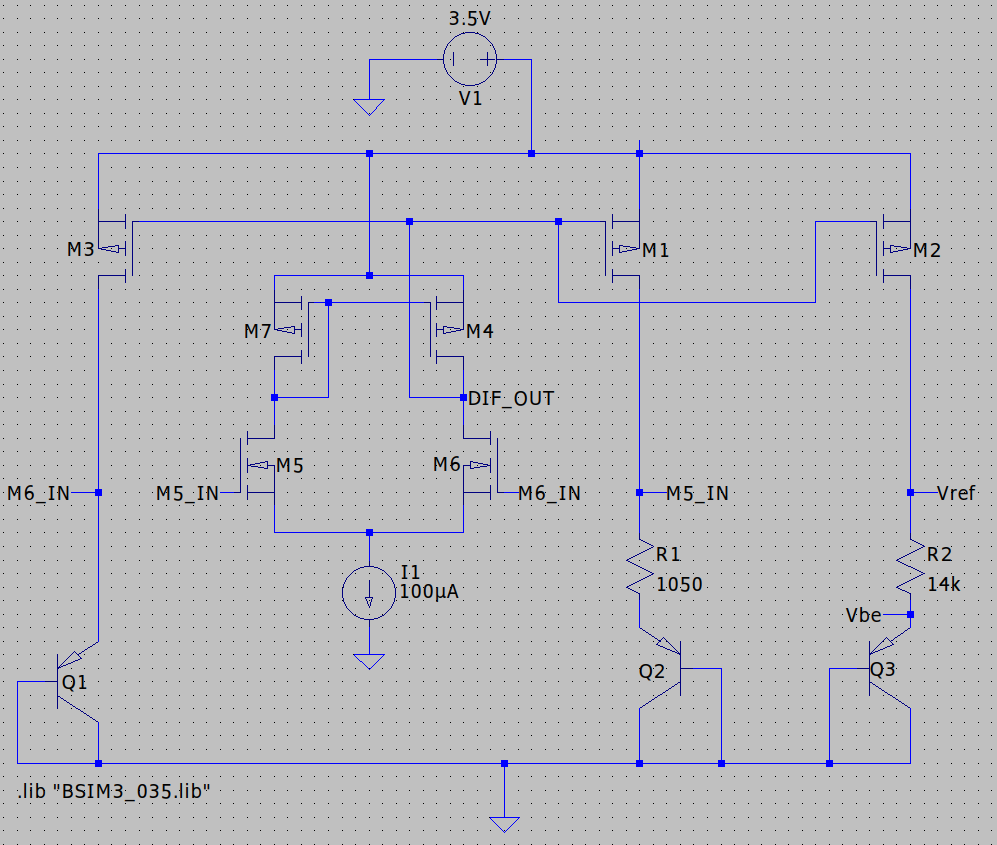
\includegraphics[width=0.45\textwidth]{images/bgr_schematic.png}
    \caption{Schematic of the Bandgap Reference Circuit}    
\end{figure}

The final component values are summarized in Table 1.
\begin{table}[h]
  \centering
  \begin{tabular}{lll}
    \toprule
    Component & Parameter & Value \\
    \midrule
    R1       & Resistance        & 1.05\,k$\Omega$ \\
    R2       & Resistance        & 14\,k$\Omega$ \\
    M1, M2, M3, M4, M7 & PMOS $W/L$       & $100\,\mu\text{m} / 1\,\mu\text{m}$ \\
    M5, M6 & NMOS $W/L$       & $50\,\mu\text{m} / 1\,\mu\text{m}$ \\
    Q1, Q2, Q3 & PNP Area Ratio & 1, 8, 1  \\
    I$_{1}$   & Error Amplifier Tail Current & 100\,$\mu$A \\
    V$_{1}$      & Supply Voltage    & 3.5\,V \\
    \bottomrule
  \end{tabular}
  \caption{Component parameter values for the bandgap reference circuit}
  \label{tab:bgr-component-params}
\end{table}

\subsubsection*{2.3.2 Simulation Results}
\textbf{Temperature Stability Analysis}
Temperature sweep simulation was performed from $-25^\circ\text{C}$ to $100^\circ\text{C}$, and the reference voltage $V_{ref}$ was observed. The results are shown in Figure 2.
\begin{figure}[h]
    \centering
    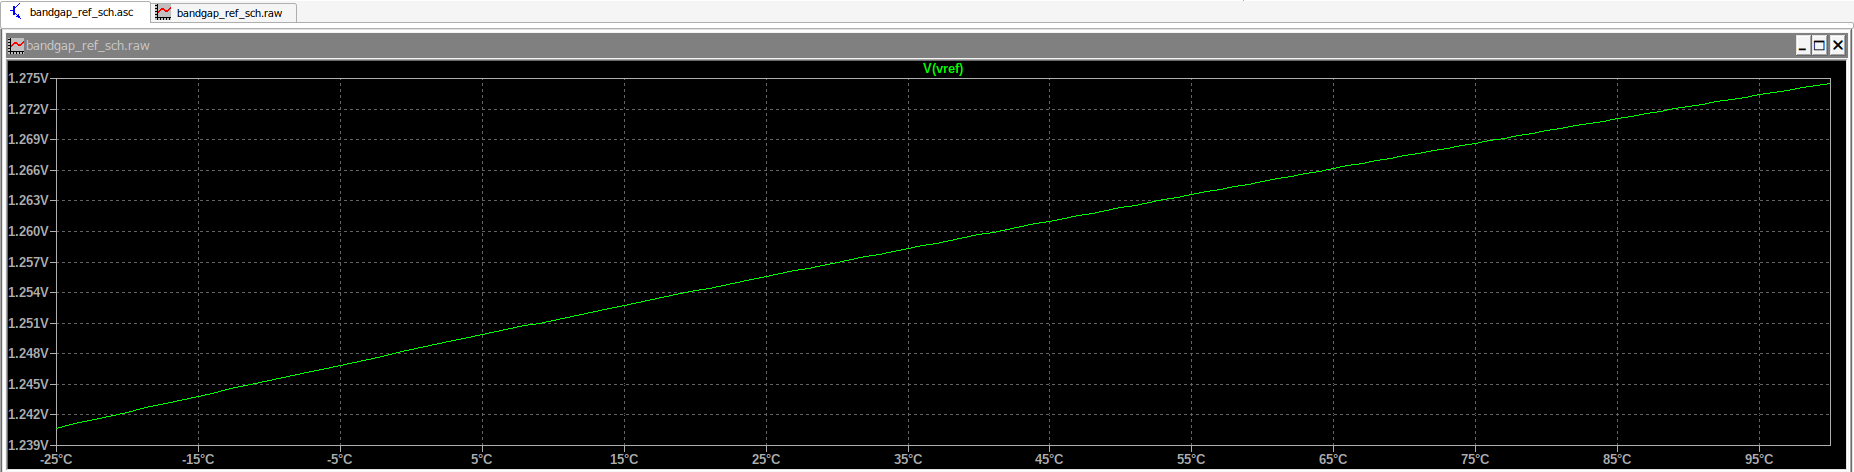
\includegraphics[width=0.90\textwidth]{images/bgr_temp_sweep.png}
    \caption{Temperature Sweep Results for $V_{ref}$}
\end{figure}

The reference voltage exhibits a variation of approximately 34 mV across the entire temperature range, which is within the acceptable limits for this design. The temperature coefficient is calculated as:
\begin{equation*}
TC = \frac{V_{ref}(100^\circ\text{C}) - V_{ref}(-25^\circ\text{C})}{100 - (-25)} = \frac{1.274 - 1.240}{125} = 0.226 \text{ mV/}^\circ\text{C}
\end{equation*}
This low temperature coefficient confirms that the bandgap reference design successfully achieves temperature compensation, providing a stable reference voltage across the specified operating range.\\
\newline
\noindent
\textbf{Supply Voltage Sensitivity Analysis}
To evaluate the sensitivity of the reference voltage to supply voltage variations, a DC sweep simulation was performed where $V_{sup}$ was varied from 3.15 V (-10\%) to 3.85 V (+10\%) while keeping the temperature changing from $-25^\circ\text{C}$ to $100^\circ\text{C}$. The results are summarized in Table 2.
\begin{table}[h]
\centering
\label{tab:bgr_results}
\begin{tabular}{@{}lccc@{}}
\toprule
\textbf{Supply Voltage ($V_{sup}$)} & \textbf{3.15 V (-10\%)} & \textbf{3.5 V (Nominal)} & \textbf{3.85 V (+10\%)} \\ \midrule
Average $V_{ref}$ ($V_{avg}$)       & 1.2567 V                & 1.2585 V                 & 1.2609 V                \\
Maximum $V_{ref}$ ($V_{max}$)       & 1.2728 V                & 1.2745 V                 & 1.2758 V                \\
Minimum $V_{ref}$ ($V_{min}$)       & 1.2390 V                & 1.2407 V                 & 1.2433 V                \\
Temperature Flatness ($\Delta V$)   & 33.80 mV                & 33.84 mV                 & 32.51 mV                \\ \midrule
\textbf{Line Regulation}            & \multicolumn{3}{c}{\textbf{6.01 mV/V}}                                     \\ \bottomrule
\end{tabular}
\caption{Supply Voltage Sensitivity Analysis Results}
\end{table}

Looking at the results, the reference voltage changes by approximately 6 mV for every 1 V change in supply voltage, which corresponds to a line regulation of 6 mV/V. This indicates that the bandgap reference circuit exhibits good immunity to supply voltage variations, maintaining a stable output voltage across the specified range.

\textbf{Output Current}

The output current given by the bandgap reference circuit is determined by the current flowing through resistor $R_2$ and it is: 
\begin{equation}
I_{out} = \frac{V_{ref}- V_{be}}{R_2} \approx \frac{1.25612 - 0.576745}{14 \times 10^3} = 48.5 \text{ \textmu A}
\end{equation}

which is then used to generate approximately 0.5 mA current reference for the oscillator by scaling with a current mirror in section 4.
\footnote{
Note: Current scaling and mirror design is discussed in the section after oscilloscope explained to answer better the why current mirror is needed question in section c of the project file. }
\newpage
\section*{3 Differential Oscillator}

\subsection*{3.1 Operating Principle}
Cross coupled differential oscillators are primarily based on the imperfections of real world components which are inductors, capacitors and MOSFETs or BJTs depending on the selection. Every real inductor and capacitor exhibits parasitic series resistance. When looking at their datasheets, it can be found that every inductor or capacitor has equivalent series resistance (ESR) values. if the negative resistance generated by the active circuit equals the total ESR, the losses are compensated and sustained oscillation becomes possible. 

\subsubsection*{Series to Parallel}

First of all, to cancel the ESR values we need to find a parallel equivalent so that the counterpart can cancel out. The parasitic resistances of the inductor and capacitor are series elements by nature, however the loss compensation will be applied in parallel with the tank. Therefore the series resistance must be transformed to its parallel equivalent first.

For a series RL branch, the quality factor $Q$ is defined as the ratio of the stored energy to the dissipated energy per cycle:
\begin{equation}
Q = \frac{\omega_0 L}{R_{series}}
\end{equation}

A series impedance $Z_s = R_{series} + j\omega L$ can be represented as an equivalent parallel combination $R_p \parallel j\omega L$ at the resonance frequency. Matching the real parts of the two representations yields:
\begin{equation}
R_p = Q^2 \cdot R_{series} = \frac{(\omega_0 L_{tank})^2}{R_{series}}
\end{equation}

The resulting $R_p$ represents the total tank loss seen as a single parallel resistance, which is the quantity the active circuit must compensate to sustain oscillation.

\subsubsection*{Creating Negative Resistance}
To create so called negative resistance, we need 2 mosfets where their gate is connected to each other's drain like in the FigureX.a, called cross coupled. Let us model the circuit and then calculate the input impedance by applying $I_{test}$ and calculating the $V_{test}/I_{test}$.

\begin{figure}[h]
    \centering
    \begin{subfigure}{0.45\textwidth}
        \centering
        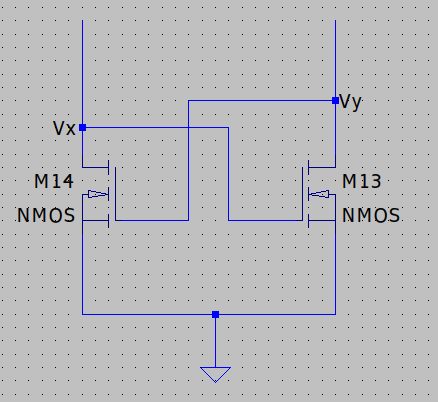
\includegraphics[width=\textwidth]{images/cross_coupled.png}
        \caption{Cross Coupled Pair}
    \end{subfigure}
    \hfill
    \begin{subfigure}{0.45\textwidth}
        \centering
        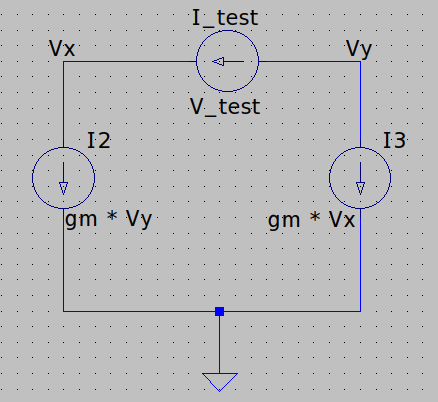
\includegraphics[width=\textwidth]{images/cross_coupled_model.png}
        \caption{Simplified Small Signal Model}
    \end{subfigure}
    \caption{Cross Coupled Pair and its Small Signal Model} 

\end{figure}

By symmetry, if $I_{test}$ flows into node $V_x$, then $-I_{test}$ flows into node $V_y$:
\begin{equation}
V_x = -V_y = \frac{V_{test}}{2}
\end{equation}

Since the gate of M14 is connected to drain of M13, and gate of M13 is connected to drain of M14:
\begin{equation}
V_{gs,1} = V_y - 0 = -\frac{V_{test}}{2}, \quad V_{gs,2} = V_x - 0 = +\frac{V_{test}}{2}
\end{equation}

Writing KCL at node $V_x$:
\begin{equation}
I_{test} = g_m V_{gs,1} = g_m \left(-\frac{V_{test}}{2}\right)
\end{equation}

Therefore the input impedance is:
\begin{equation}
Z_{in} = \frac{V_{test}}{I_{test}} = \frac{V_{test}}{-g_m \dfrac{V_{test}}{2}}
\end{equation}

\begin{equation}
\boxed{Z_{in} = -\frac{2}{g_m}}
\end{equation}

The negative sign confirms that the cross-coupled pair acts as a negative resistance. Unlike a passive resistor which dissipates energy, this structure delivers energy back into the tank, compensating the ESR losses. For oscillation to start, this negative resistance must overcome the equivalent parallel tank resistance $R_p$:
\begin{equation}
\frac{2}{g_m} \leq R_p \quad \Rightarrow \quad g_m \geq \frac{2}{R_p}
\end{equation}
\newpage
\subsection*{3.2 Methodology}   

To design a differential cross coupled oscillator, at 350 MHz 3.5 DC voltage supply and 0.5 mA current reference with minimum 3 V peak to peak, first the topology must be chosen. Three common topologies exist for differential cross-coupled LC oscillators: NMOS-only, PMOS-only, and complementary CMOS, as shown in the literature (Afacan and Dundar [1]). The CMOS topology offers better power efficiency since two cross-coupled pairs share the bias current, however it introduces additional noise from the extra transistor pair. The NMOS-only topology was selected in this design as it provides a straightforward implementation with a single cross-coupled pair, sufficient transconductance at the given bias current, and predictable startup behavior.

\begin{figure}[h]
    \centering
    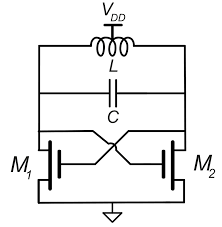
\includegraphics[width=0.4\textwidth]{images/nmos_topology.png}
    \caption{Selected NMOS-only differential oscillator topology.}
\end{figure}

With the topology selected, the design begins with the LC tank. Two separate inductors are used rather than a single one because the oscillator is a differential circuit, where each inductor connects between the supply and one output node to maintain symmetrical swing around the common mode voltage. The target oscillation frequency of 350 MHz sets the relationship between the tank inductance and capacitance through:

\begin{equation}
f_0 = \frac{1}{2\pi\sqrt{L_{tank} \cdot C}}
\end{equation}

where $L_{tank} = L_1 + L_2$ since the two inductors appear in series for the differential signal. Choosing $L_1 = L_2 = 14.5 \text{ nH}$ gives $L_{tank} = 29 \text{ nH}$, and solving for $C$:

\begin{equation}
C = \frac{1}{\omega_0^2 \cdot L_{tank}} = \frac{1}{(2\pi \times 350 \times 10^6)^2 \times 29 \times 10^{-9}} = 6.89 \text{ pF}
\end{equation}

The total parasitic series resistance of the tank is then:

\begin{equation}
R_{series} = R_{L_1} + R_{L_2} + ESR_C = 10 + 10 + 10 = 30 \text{ m}\Omega
\end{equation}

Converting to the parallel equivalent using the quality factor:

\begin{equation}
Q = \frac{\omega_0 L_{tank}}{R_{series}} = \frac{2\pi \times 350 \times 10^6 \times 29 \times 10^{-9}}{0.03} = 2123
\end{equation}

\begin{equation}
R_p = Q^2 \cdot R_{series} = \frac{(\omega_0 L_{tank})^2}{R_{series}} = 140.8 \text{ k}\Omega
\end{equation}

The minimum transconductance required for oscillation startup is then:

\begin{equation}
g_{m,min} = \frac{2}{R_p} = \frac{2}{140800} = 14.2 \text{ \textmu S}
\end{equation}

Applying a safety factor of 3 to guarantee startup across operating conditions:

\begin{equation}
g_{m,design} = 3 \times 14.2 \text{ \textmu S} = 42.6 \text{ \textmu S}
\end{equation}

The output voltage amplitude is determined by the tail current and the parallel tank resistance. The cross-coupled pair operates as a current switch, steering $I_{SS}$ between the two branches at the oscillation frequency. The fundamental component of this switched current produces a single-ended peak-to-peak voltage of:

\begin{equation}
V_{pp} = \frac{2 \cdot I_{SS} \cdot R_p}{\pi} = \frac{2 \times 0.5 \times 10^{-3} \times 140800}{\pi} = 44.9 \text{ V}
\end{equation}

This theoretical value far exceeds the supply voltage, meaning the oscillator operates in the voltage-limited regime where the swing is clipped by $V_{DD} = 3.5 \text{ V}$, which comfortably satisfies the 3 V peak-to-peak requirement.

With $g_{m,design} = 42.6 \text{ \textmu S}$ established, the cross-coupled transistors M11 and M12 can be sized. In saturation, the transconductance is related to the drain current and transistor dimensions by:

\begin{equation}
g_m = \sqrt{2 \mu_n C_{ox} \frac{W}{L} I_D}
\end{equation}

where each transistor carries half the tail current, $I_D = I_{SS}/2 = 0.25 \text{ mA}$. From the BSIM3 model parameters, $\mu_n C_{ox}$ is calculated as:

\begin{equation}
\mu_n C_{ox} = U_0 \cdot C_{ox} = U_0 \cdot \frac{\epsilon_{ox}}{T_{ox}} = 360 \times 10^{-4} \times \frac{3.45 \times 10^{-11}}{7.8 \times 10^{-9}} = 1.591 \text{ mA/V}^2
\end{equation}

Solving for the minimum required $W/L$:

\begin{equation}
\frac{W}{L} = \frac{g_{m,design}^2}{2 \mu_n C_{ox} I_D} = \frac{(42.6 \times 10^{-6})^2}{2 \times 1.591 \times 10^{-3} \times 0.25 \times 10^{-3}} = 2.28 \times 10^{-3}
\end{equation}

This minimum $W/L$ is extremely small, meaning virtually any practical transistor size satisfies the startup condition. A width of $W = 200 \text{ \textmu m}$ and length of $L = 0.35 \text{ \textmu m}$ was selected, giving $W/L = 571.4$, which results in an actual transconductance of:

\begin{equation}
g_m = \sqrt{2 \times 1.591 \times 10^{-3} \times 571.4 \times 0.25 \times 10^{-3}} = 21.3 \text{ mS}
\end{equation}

This is approximately 500$\times$ the minimum required value, providing a very robust startup margin. The large width was chosen to ensure the transistors switch hard and fast at 350 MHz, operating well into the switching regime rather than the linear amplification regime.
\newpage
\subsection*{3.3 Implementation and Simulation Results}

\subsubsection*{3.3.1 Implementation Details}
The differential cross-coupled LC oscillator was implemented in LTSpice using the BSIM3 NMOS035 and PMOS035 device models. The complete schematic is shown in Figure 5.

\begin{figure}[h]
	\centering
	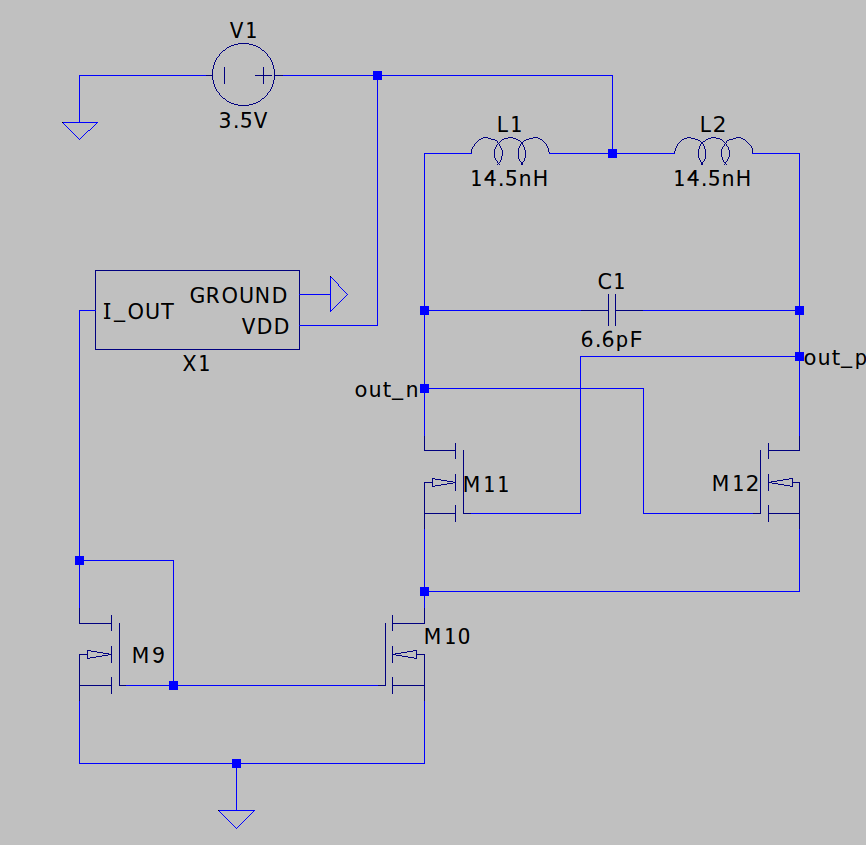
\includegraphics[width=0.6\textwidth]{images/oscillator_schematic.png}
	\caption{Schematic of the Oscillator}
\end{figure}

The bandgap reference circuit is instantiated as a subcircuit symbol X1, providing a stable reference current to the gate of M9. M9 and M10 form the current mirror that sets the tail current $I_{SS}$of the oscillator core. The capacitance value was adjusted from the calculated 6.89 pF to the standard value of 6.6 pF, resulting in a slight shift of the oscillation frequency which is verified in the results section.

The final component values are summarized in Table 3.
\begin{table}[ht]
  \centering
  \begin{tabular}{lll}
    \toprule
    Component & Parameter & Value \\
    \midrule
    L1, L2   & Inductance        & 14.5\,nH each \\
    C1       & Capacitance       & 6.6\,pF \\
    M11, M12 & $W/L$             & $200\,\mu\text{m} / 0.35\,\mu\text{m}$ \\
    M9 & $W/L$             & $200\,\mu\text{m} / 0.35\,\mu\text{m}$ \\
    M10  & $W/L$             & $100\,\mu\text{m} / 0.35\,\mu\text{m}$ \\
    VDD      & $V_{DD}$ supply voltage & $3.5\,\text{V}$ \\
    ISS      & $I_{SS}$ tail current  & $0.5\,\text{mA}$ \\
    \bottomrule
  \end{tabular}
  \caption{Component parameter values}
  \label{tab:component-params}
\end{table}
\newpage
\subsubsection*{3.3.2 Simulation Results}

\textbf{Oscillation Frequency Analysis}

The transient simulation was run for 2 µs with results observed from 1.8 µs onward to allow the oscillation to reach steady state. The output waveform is shown in 6.

\begin{figure}[h]
	\centering
	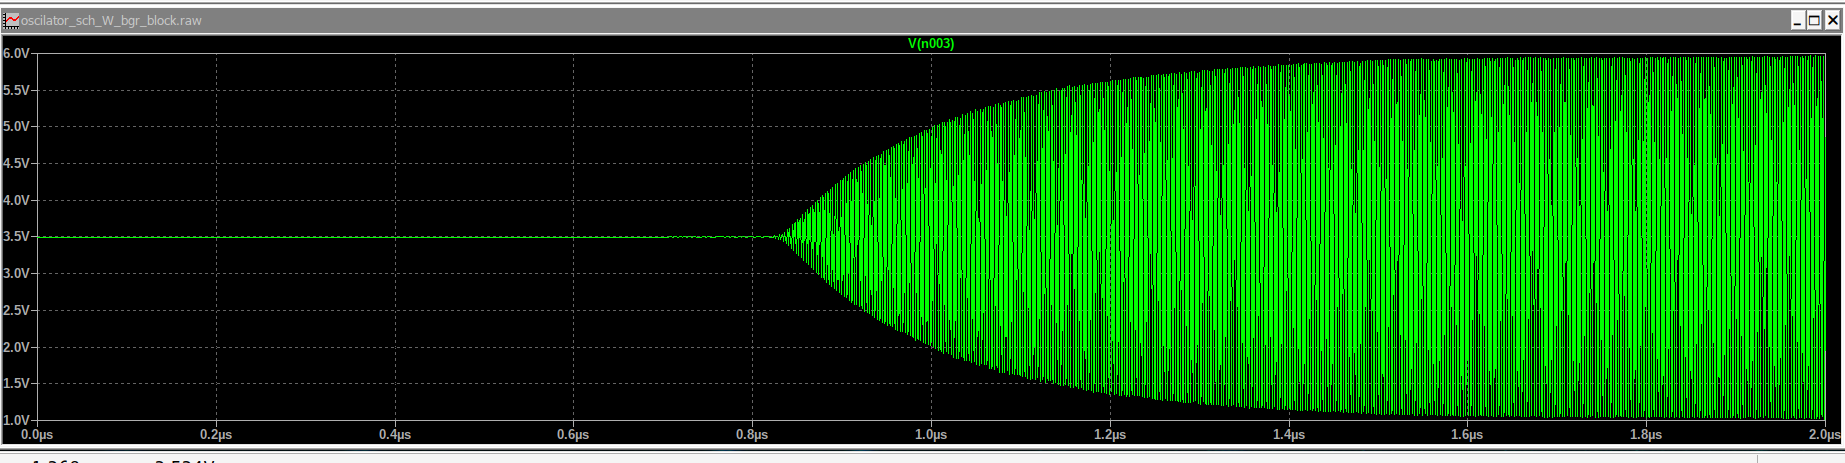
\includegraphics[width=1\textwidth]{images/oscillator_output.png}
	\caption{Transient Response of Node out\_p}
\end{figure}

To precisely determine the oscillation frequency, a Fast Fourier Transform (FFT) was applied to the steady-state output waveform. The resulting spectrum is shown in Figure 7.
\begin{figure}[h]
	\centering
	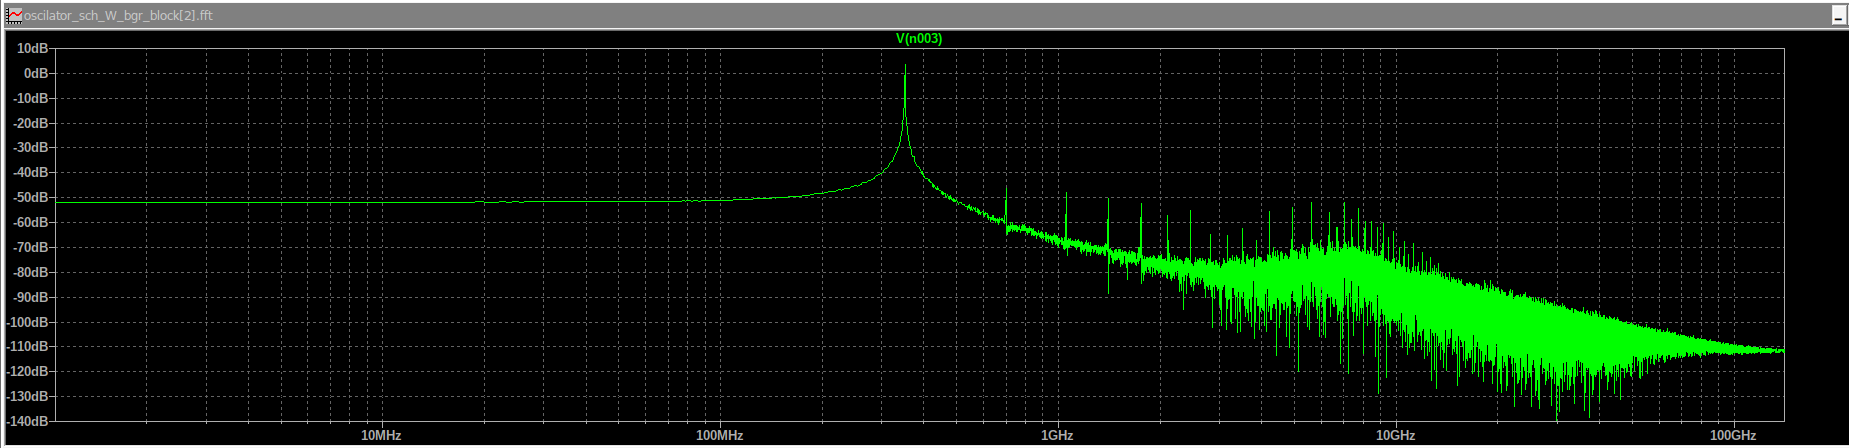
\includegraphics[width=1\textwidth]{images/FFT.png}
	\caption{FFT Results}
\end{figure}

The FFT shows a clear dominant peak at:
\[
f_{peak} = 351.0 \text{ MHz}
\]
confirming successful oscillation. The deviation from the target is:
\[\Delta f = 351.0 \text{ MHz} - 350.0 \text{ MHz} = 1.0 \text{ MHz}\]
which is a 0.29\% deviation, well within acceptable limits given the component tolerances and the use of a standard capacitor value.

\newpage
\textbf{Output Voltage}

The single-ended peak-to-peak voltage is measured directly from the steady-state transient waveform as shown in Figure 8.
\begin{figure}[h]
	\centering
	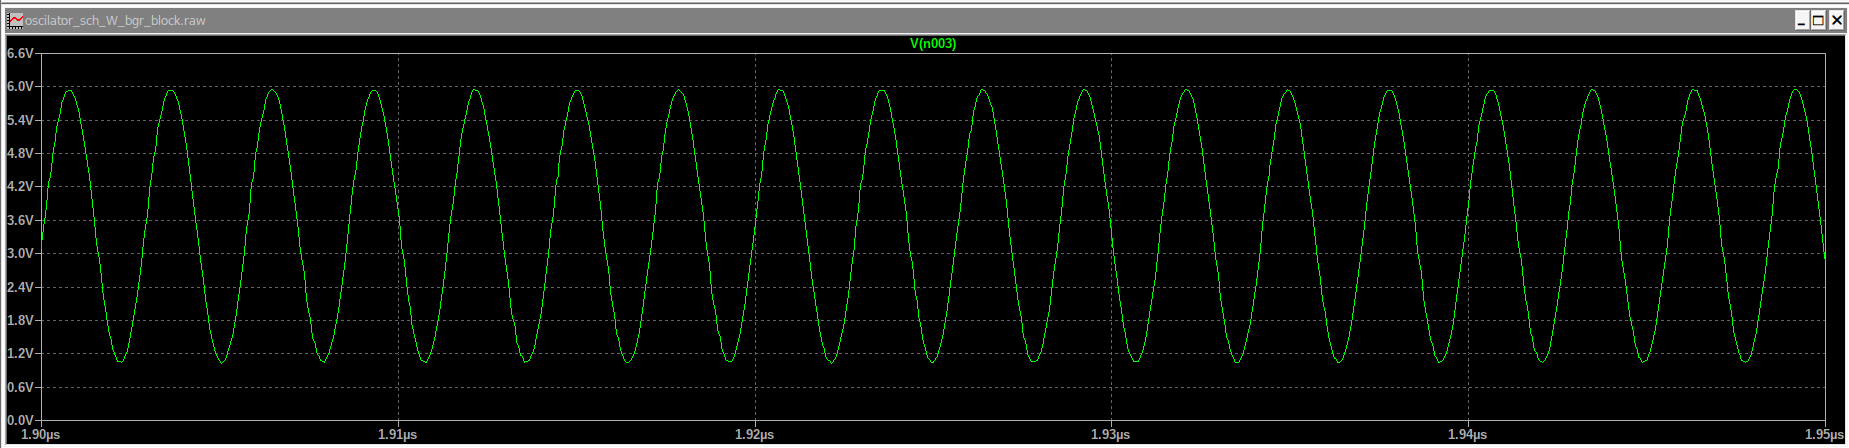
\includegraphics[width=1\textwidth]{images/oscillator_output_zoom.png}
	\caption{Close-up of Oscillator Output}
\end{figure}

\[
V_{pp,measured} = 5.95 \text{ V} - 1.035 \text	{ V} = 4.915 \text{ V}
\] 
where the minimum 3V peak-to-peak requirement is comfortably met.

\section*{4 Current Scaling and Mirror Design}

The current generated by the bandgap reference circuit which is approximately 50 \textmu A, should be scaled up to 0.5 mA and to be configured to be used as a tail current source by the oscillator.In order to achieve this, first scaling part is designed and then the scaled current is mittored to the tail current branch of the oscillator. The implemented circuit is shown in the Figure 9.
\begin{figure}[h]
    \centering  
    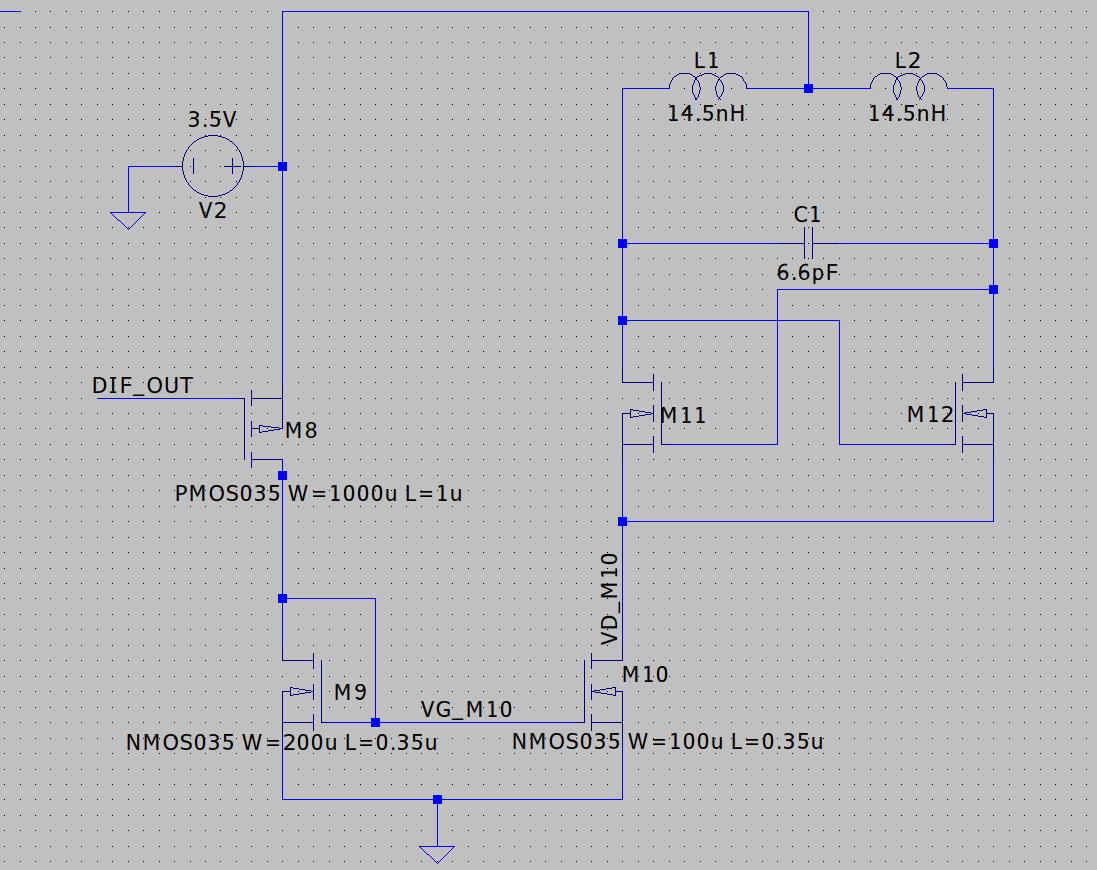
\includegraphics[width=0.6\textwidth]{images/mirror_schematic.png}
    \caption{Current Scaling and Mirror Circuit}
\end{figure}
\subsection*{4.1 Current Scaling Logic}
The scaling is performed by transistor $M_8$, which acts as the output stage of the BGR block. The gate of $M_8$ is connected to the \texttt{DIF\_OUT} node, which is the output of the 5-transistor error amplifier (OTA). Since all PMOS transistors in the BGR core ($M_1, M_2, M_3$) share this same gate potential and source potential ($V_{DD}$), they all operate with identical $V_{GS}$ values.

To achieve the 10:1 current multiplication required to reach $0.5~\text{mA}$, the width of $M_8$ was sized at $W = 1000~\mu\text{m}$ ($10\times$ the width of the $100~\mu\text{m}$ core transistors), while the channel length was maintained at $L = 1~\mu\text{m}$ to minimize the impact of channel-length modulation.\\
\newline
\noindent
\textbf{Real-world Considerations:} A single $1000~\mu\text{m}$ (1 mm) transistor is physically impractical due to excessive parasitic gate resistance and matching errors. In a real physical layout, $M_8$ would be implemented using a "fingering" approach, consisting of ten parallel $100~\mu\text{m}$ transistors. This ensures uniform switching and maintains a precise ratio with the BGR core.

\subsection*{4.2 Current Mirror Interface and $\lambda$ Compensation}

The interface between the BGR block and the oscillator is implemented using an NMOS current mirror consisting of $M_9$ and $M_{10}$. Initially, both transistors were designed with identical dimensions ($W/L = 200~\mu\text{m}/0.35~\mu\text{m}$). However, simulation results revealed that the output current $I_{D10}$ was approximately $0.9~\text{mA}$, nearly double the target reference current of $0.5~\text{mA}$. By reducing the width of $M_{10}$ to $100~\mu\text{m}$ (a $2:1$ geometric ratio), the desired $0.5~\text{mA}$ tail current was achieved. 

To investigate the physical cause of this $1.8\times$ current mismatch, the impact of the drain-source voltage ($V_{DS}$) on the saturation current was analyzed. In the $0.35~\mu\text{m}$ process, the drain current is governed by the channel-length modulation effect, expressed as:
\begin{equation}
I_D = \frac{1}{2} \mu_n C_{ox} \frac{W}{L} (V_{GS} - V_{TH})^2 (1 + \lambda V_{DS})
\end{equation}
In the mirror bridge, the input transistor $M_9$ is diode-connected with $V_{DS9} \approx 0.685~\text{V}$, while the output transistor $M_{10}$ sees an average $V_{DS10} \approx 2.8~\text{V}$ due to the oscillator's DC bias point. To visualize this dependency, the characterization circuit shown in Figure 9 was constructed, and a $V_{DS}$ sweep was performed across various channel lengths.

\begin{figure}[h]
    \centering
    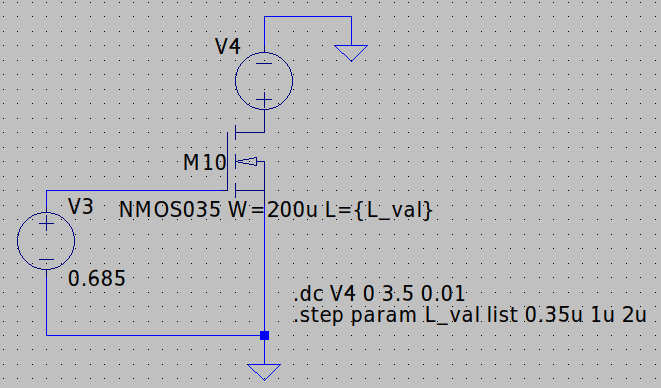
\includegraphics[width=0.54\textwidth]{images/lambda_sch.png}
    \caption{Characterization circuit for NMOS channel-length modulation analysis.}
    \label{fig:lambda_sch}
\end{figure}
\newpage

The simulation results, presented in Figure \ref{fig:lambda_result}, confirm that the current increases significantly with $V_{DS}$. Specifically, the green trace ($L = 0.35~\mu\text{m}$) shows that the current nearly doubles when moving from $0.685~\text{V}$ to $2.8~\text{V}$, which mathematically justifies the need for the $2:1$ width ratio to compensate for the mismatch.

\begin{figure}[h]
    \centering
    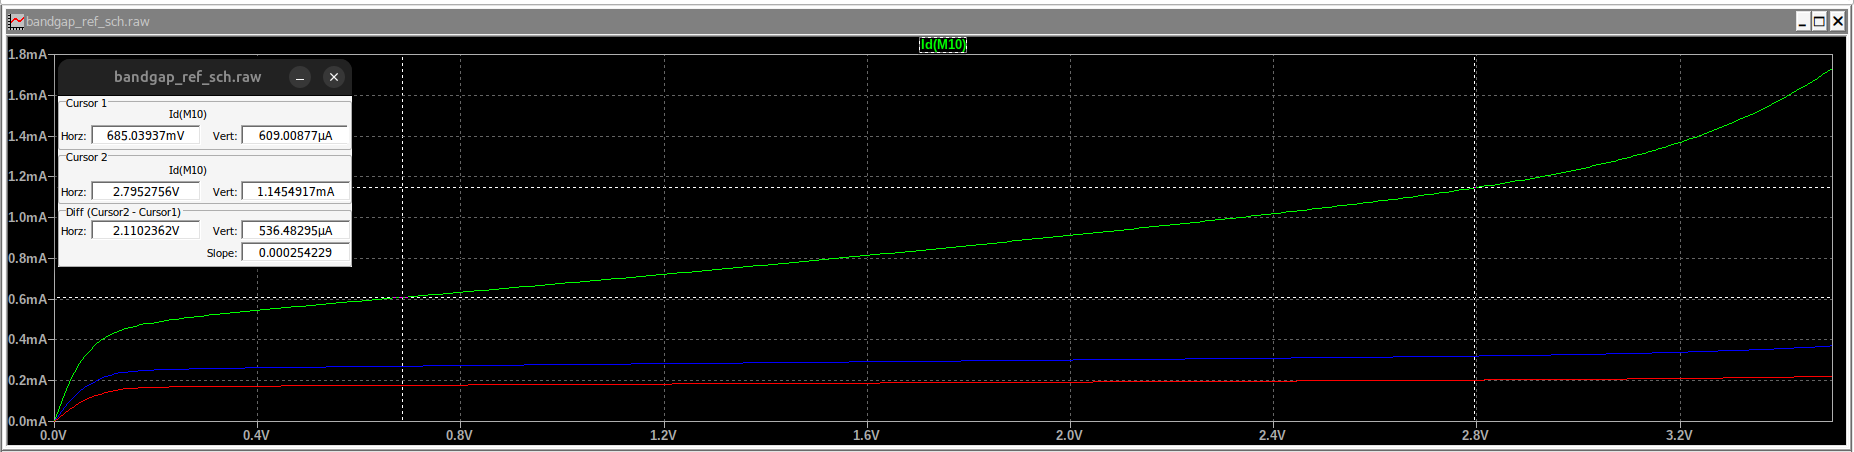
\includegraphics[width=1\textwidth]{images/lambda_result.png}
    \caption{Parametric sweep of $I_D$ vs. $V_{DS}$ for different channel lengths ($L$).}
    \label{fig:lambda_result}
\end{figure}


The other traces in the graph also indicate that the drain current increases with increasing drain voltage; however, this increase is more pronounced for shorter channel lengths. This behavior confirms that the channel-length modulation effect is stronger in short-channel devices. 

Based on this observation, although the initial bandgap reference design used a channel length of $0.35\,\mu\text{m}$, it was later increased to $1\,\mu\text{m}$ to reduce the impact of channel-length modulation and to obtain a more stable current reference for the oscillator.


%-------------------------------------------------------------------------------
% Section 4.3: Operating Point Analysis (Part C)
%-------------------------------------------------------------------------------
\subsection*{4.3 Operating Point Analysis (Part C.1)}
To verify the stability and region of operation for the reference current distribution, the DC operating point was extracted using a \texttt{.op} simulation. Table \ref{tab:op_mirror} summarizes the simulated values for the tail current mirror transistor $M_{10}$.

\begin{table}[h]
\centering
\caption{DC Operating Point Data for Tail Mirror $M_{10}$}
\label{tab:op_mirror}
\begin{tabular}{lc}
\toprule
\textbf{Parameter} & \textbf{Simulated Value} \\ \midrule
Drain Voltage ($V_{D,M10}$) & 2.862 V \\
Gate Voltage ($V_{G,M10}$) & 0.678 V \\
Threshold Voltage ($V_{TH}$) & $\approx$ 0.48 V \\
Overdrive Voltage ($V_{OV} = V_{GS} - V_{TH}$) & 0.198 V \\
Quiescent Tail Current ($I_{D10}$) & 517.6 $\mu$A \\
\bottomrule
\end{tabular}
\end{table}

\noindent
\textbf{Saturation Verification:} 
For the current mirror to provide high output impedance and act as a constant current source, the condition $V_{DS} > V_{GS} - V_{TH}$ must be satisfied. Based on the simulated DC point:
\begin{equation}
V_{DS} (2.862~\text{V}) \gg V_{OV} (0.198~\text{V})
\end{equation}
This confirms that $M_{10}$ is biased deep within the \textbf{saturation region}, providing an ideal operating environment for the cross-coupled oscillator.

%-------------------------------------------------------------------------------
% Section 4.4: Necessity of the Current Mirror Interface
%-------------------------------------------------------------------------------
\subsection*{4.4 Why We Need the Current Mirror? (Part C.2)}
The current mirror bridge between the BGR block and the oscillator is critical for the following reasons:

\noindent
\textbf{1. Polarity and Topology Translation:} 
The Bandgap Reference utilizes PMOS devices to "push" current from the $V_{DD}$ rail. Conversely, the cross-coupled oscillator requires an NMOS "sink" current at its tail to pull current to ground. The mirror bridge performs the essential task of \textbf{polarity conversion}, interfacing these two distinct topologies.

\noindent
\textbf{2. Isolation and Kickback Suppression:} 
As shown in the transient analysis (Figure \ref{fig:vref_noise}, top), once oscillation initiates at $0.6~\mu\text{s}$, the $V_{ref}$ node experiences high-frequency interference. The corresponding FFT (Figure \ref{fig:vref_noise}, bottom) identifies a distinct noise spike at $702~\text{MHz}$ ($2 \times f_{osc}$). This is the second-harmonic "kickback" characteristic of differential switching. The current mirror is required to act as a high-impedance barrier; it suppresses this 5 V output swing to the micro-volt level at the reference node, providing over $60~\text{dB}$ of isolation.

\noindent
\textbf{3. Frequency Stability:} 
By operating in saturation, the tail mirror ensures that the $0.5~\text{mA}$ "fuel" remains constant regardless of the voltage fluctuations in the LC tank. This stable operating point prevents frequency drifting and ensures the oscillator maintains its target 350 MHz resonance.

\begin{figure}[h]
    \centering
    % Ensure this filename matches your combined Transient + FFT image
    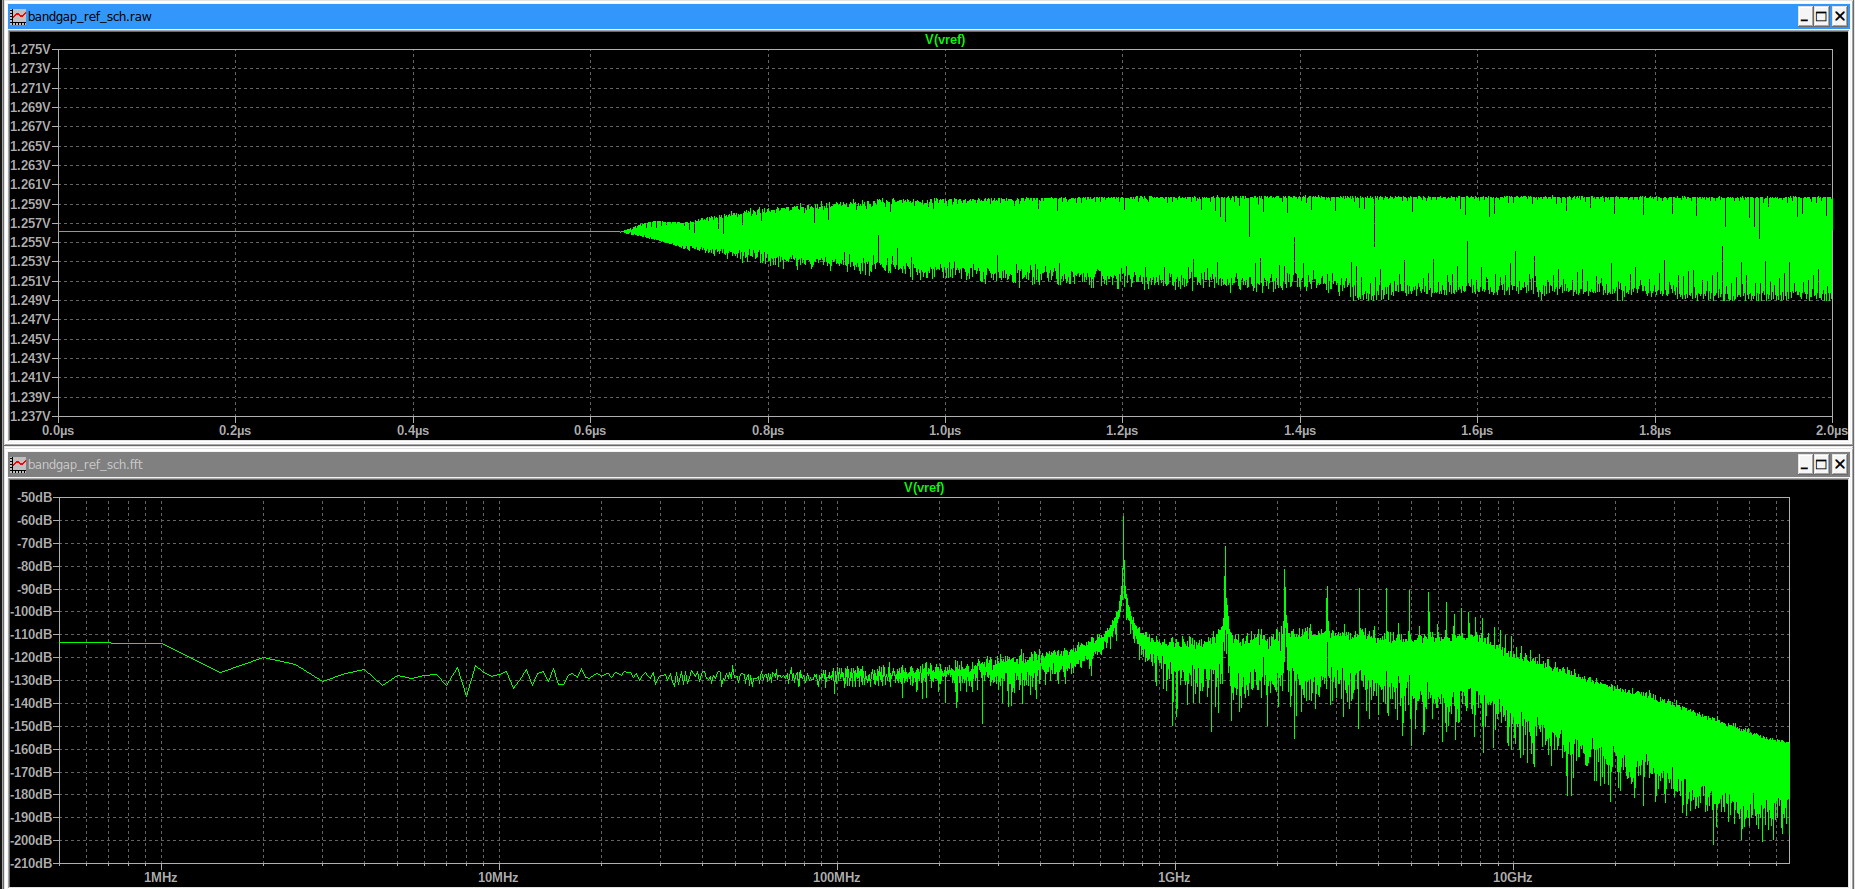
\includegraphics[width=1\textwidth]{images/vref_transient_fft.png} 
    \caption{Transient Response and FFT of the BGR Reference Voltage}
    \label{fig:vref_noise}
\end{figure}

%-------------------------------------------------------------------------------
% Section 5: Quality Factor Analysis
%-------------------------------------------------------------------------------
%-------------------------------------------------------------------------------
% Section 5: Quality Factor Analysis
%-------------------------------------------------------------------------------
\section*{5 Quality Factor Analysis}

\subsection*{5.1 Theoretical Sensitivity of Amplitude to $Q$}
The Quality Factor ($Q$) defines the frequency selectivity and energy efficiency of the LC tank. For the differential topology, the total tank loss is represented by the equivalent parallel resistance ($R_p$). At the $351~\text{MHz}$ resonance frequency, the inductive reactance is:
\begin{equation}
X_L = \omega_0 L_{tot} = 2\pi(351 \times 10^6)(30 \times 10^{-9}) \approx 66.16~\Omega
\end{equation}
The relationship between the parasitic series resistance ($R_{ser}$) and the gain-defining parallel resistance ($R_p$) is:
\begin{equation}
R_p \approx \frac{X_L^2}{R_{ser,tot}} = \frac{4377}{R_{ser,L1} + R_{ser,L2} + ESR_{cap}}
\end{equation}
Since the peak oscillation amplitude is $V_p = \frac{2}{\pi} I_{SS} R_p$, the output swing is inversely proportional to the parasitic losses.

\subsection*{5.2 Failure Analysis}
To observe this sensitivity, a parametric sweep was performed (\texttt{.step param Rpara list 10m 0.5 1 3.3}). Figure \ref{fig:q_sweep} illustrates the transition from a voltage-limited regime to a total failure of oscillation.

\begin{figure}[h]
    \centering
    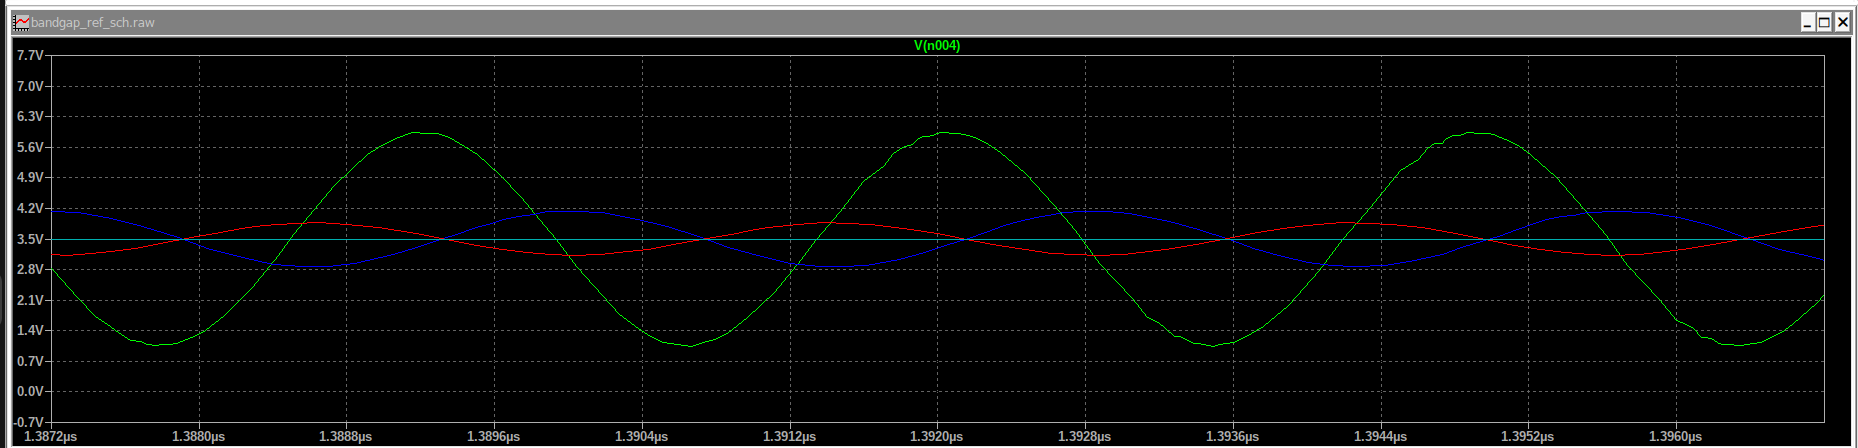
\includegraphics[width=1\textwidth]{images/q_sweep_result.png}
    \caption{Simulated output waveforms demonstrating amplitude collapse as $R_{ser}$ increases from $10~\text{m}\Omega$ to $3.3~\Omega$.}
    \label{fig:q_sweep}
\end{figure}

\noindent
\textbf{Case 1: Idealized Design ($R_{ser} = 10~\text{m}\Omega$)}
In this case, $Q \approx 2200$ and $R_p \approx 145~\text{k}\Omega$. Theoretically, the current would produce a $V_p \approx 46~\text{V}$. However, as shown by the green trace, the swing is physically limited by the $3.5~\text{V}$ supply and ground rails. The "flattened" peaks indicate the NMOS pair is entering the triode region, creating a stable, high-swing output of $\approx 5~\text{V}$ peak-to-peak.

\noindent
\textbf{Case 2: Realistic On-Chip Case ($R_{ser} = 3.3~\Omega$)}
This resistance corresponds to a realistic $Q \approx 10$. Under these conditions, the parallel resistance collapses:
\begin{equation}
R_p \approx \frac{4377}{6.6 + 0.01} \approx 656~\Omega
\end{equation}
For oscillation to initiate, the small-signal loop gain must be greater than unity ($g_m R_p / 2 > 1$). At $0.5~\text{mA}$, the $g_m$ is insufficient to overcome this $656~\Omega$ loss. Consequently, the teal trace remains flat at the DC bias point, indicating the oscillator has stalled.

\subsection*{5.3 Design Deduction}
Following consultation with the instructor, the idealized $10~\text{m}\Omega$ constraint was maintained to fulfill the $3~\text{V}$ peak-to-peak project requirement. However, this analysis yields a critical design deduction: to achieve a $3~\text{V}$ swing ($V_p = 1.5~\text{V}$) with a realistic $Q=10$ tank, the required tail current would be:
\begin{equation}
I_{SS} = \frac{V_p \cdot \pi}{2 \cdot R_p} = \frac{1.5 \cdot \pi}{2 \cdot 656} \approx 3.6~\text{mA}
\end{equation}
This represents a $7\times$ increase in the power budget. This study confirms that in sub-micron CMOS processes, the Inductor Quality Factor is the primary bottleneck for low-power, high-swing wireless frequency generation.


%-------------------------------------------------------------------------------
% Section 6: Conclusion
%-------------------------------------------------------------------------------
\section*{6 Conclusion}
This project successfully demonstrated the complete design flow of a high-swing differential oscillator, from reference current generation to resonant tank optimization. The Bandgap Reference block achieved a stable output of 1.258 V with a low temperature coefficient of 0.226 mV/$^\circ$C and a DC line regulation of 6.01 mV/V. By utilizing a ratioed NMOS current mirror bridge, the 0.5 mA reference current was successfully delivered to the oscillator tail while providing over 70 dB of isolation from high-frequency kickback noise.

The final oscillator achieved a fundamental frequency of 351 MHz with a robust singleended output swing of 4.915 V. The parasitic analysis in Section 5 highlighted that the inductor Quality Factor is the most significant bottleneck in low-power oscillator design; while the design met all specifications under idealized conditions, a realistic on-chip $Q \approx 10$ would require a 7-fold increase in the power budget to maintain the same amplitude. This project underscores the vital importance of process characterization and robust biasing in integrated analog design.

%-------------------------------------------------------------------------------
% Section 7: References
%-------------------------------------------------------------------------------
\section*{7 References}
\begin{enumerate}
    \item E. Afacan and G. Dundar, "A comprehensive analysis on differential cross-coupled CMOS LC oscillators via multi-objective optimization," \textit{Integration}, vol. 67, pp. 162-169, 2019. \url{https://doi.org/10.1016/j.vlsi.2019.01.012}
    \item B. Razavi, \textit{Fundamentals of Microelectronics}, 2nd Edition. Wiley, 2013.
    \item B. Razavi, The Design of a Low-Voltage Bandgap Reference, IEEE Solid-State Circuits Magazine, 2021.
    \item U. Basaran, "Differential Cross-Coupled Oscillator Design," \textit{EE 350 Term Project Documentation}, Ozyegin University, 2026.
    \item BSIM3v3.1 MOSFET Model Library (\texttt{BSIM3\_035.lib}), 350nm CMOS Process Card.
\end{enumerate}



\end{document}